\section{Appendix}


Include extra information in the appendix. This section will often be part of the supplemental material. Please see the call on the NeurIPS website for links to additional guides on dataset publication.

\begin{enumerate}

% \item Submission introducing new datasets must include the following in the supplementary materials:
% \begin{enumerate}
  % \item Dataset documentation and intended uses. Recommended documentation frameworks include datasheets for datasets, dataset nutrition labels, data statements for NLP, and accountability frameworks.
  % \item URL to website/platform where the dataset/benchmark can be viewed and downloaded by the reviewers.
  % \item Author statement that they bear all responsibility in case of violation of rights, etc., and confirmation of the data license.
  % \item Hosting, licensing, and maintenance plan. The choice of hosting platform is yours, as long as you ensure access to the data (possibly through a curated interface) and will provide the necessary maintenance.
% \end{enumerate}

\item To ensure accessibility, the supplementary materials for datasets must include the following:
\begin{enumerate}
  % \item Links to access the dataset and its metadata. This can be hidden upon submission if the dataset is not yet publicly available but must be added in the camera-ready version. In select cases, e.g when the data can only be released at a later date, this can be added afterward. Simulation environments should link to (open source) code repositories.
  % \item The dataset itself should ideally use an open and widely used data format. Provide a detailed explanation on how the dataset can be read. For simulation environments, use existing frameworks or explain how they can be used.
  % \item Long-term preservation: It must be clear that the dataset will be available for a long time, either by uploading to a data repository or by explaining how the authors themselves will ensure this.
  % \item Explicit license: Authors must choose a license, ideally a CC license for datasets, or an open source license for code (e.g. RL environments).
  % \item Add structured metadata to a dataset's meta-data page using Web standards (like schema.org and DCAT): This allows it to be discovered and organized by anyone. If you use an existing data repository, this is often done automatically.
  \item Highly recommended: a persistent dereferenceable identifier (e.g. a DOI minted by a data repository or a prefix on identifiers.org) for datasets, or a code repository (e.g. GitHub, GitLab,...) for code. If this is not possible or useful, please explain why.
\end{enumerate}

\item For benchmarks, the supplementary materials must ensure that all results are easily reproducible. Where possible, use a reproducibility framework such as the ML reproducibility checklist, or otherwise guarantee that all results can be easily reproduced, i.e. all necessary datasets, code, and evaluation procedures must be accessible and documented.

\item For papers introducing best practices in creating or curating datasets and benchmarks, the above supplementary materials are not required.
\end{enumerate}

Please refer to \url{https://github.com/EpistasisLab/srbench/} for the most up-to-date guide to running the benchmark study. 

\subsection{Running the Benchmark}

\subsection{Contributing a Method}
A living version of the method contribution instructions are described in the \href{https://github.com/EpistasisLab/srbench/blob/master/CONTRIBUTING.md}{Contribution Guide}.
To illustrate the simplicity of contributing a method, Figure~\ref{fig:ex_code} shows the script submitted for Bayesian Symbolic Regression~\cite{jinBayesianSymbolicRegression2020}. 
In addition to the code snippet, authors may either add their code package to the conda/pip environment, or provide an install script.
When a pull request is issued by a contributor, new methods and installs are automatically tested on a minimal version of the benchmark.  

\begin{figure}
	\DeclareTCBListing{mintedbox}{O{}m!O{}}{%
  breakable=true,
  listing engine=minted,
  listing only,
  minted language=#2,
  minted style=default,
  minted options={%
    linenos,
    gobble=0,
    breaklines=true,
    breakafter=,,
    fontsize=\footnotesize,
    numbersep=8pt,
    #1},
  boxsep=0pt,
  left skip=0pt,
  right skip=0pt,
  left=25pt,
  right=0pt,
  top=3pt,
  bottom=3pt,
  arc=5pt,
  leftrule=0pt,
  rightrule=0pt,
  bottomrule=2pt,
  toprule=2pt,
  colback=bg,
  colframe=orange!70,
  enhanced,
  overlay={%
    \begin{tcbclipinterior}
    \fill[orange!20!white] (frame.south west) rectangle ([xshift=20pt]frame.north west);
    \end{tcbclipinterior}},
  #3}
\begin{mintedbox}{python}
# method: Bayesian Symbolic Regression
# contributor: Ying Jin
# source: https://github.com/ying531/MCMC-SymReg
from bsr.bsr_class import BSR

hyper_params = []
for val, itrNum in zip([100,500,1000],[5000,1000,500]):
    for treeNum in [3,6]:
        hyper_params.append(
                    {'treeNum': [treeNum], 
                     'itrNum': [itrNum], 
                     'val': [val],
                    })
# default estimator
est = BSR(val=100, itrNum=5000, treeNum=3, alpha1=0.4, alpha2=0.4, 
          beta=-1, disp=False, max_time=2*60*60)

def complexity(est):
"""returns final model complexity"""
    return est.complexity()

def model(est):
"""returns final model as string"""
    return est.model()
\end{mintedbox}


    \caption{
        An example code contribution, defining the estimator, its hyperparameters, and functions to return the complexity and symbolic model.
    }\label{fig:ex_code} 
\end{figure}

\subsection{Additional Background and Motivation}

Eureqa is a closed-source commercial software that was acquired by DataRobot in 2017\footnote{\url{https://www.datarobot.com/nutonian/}}. 
Due to its proprietary nature and incorporation into the DataRobot platform, it is impossible to benchmark its performance while controlling for important experimental variables such as computational effort. 
However, the algorithmic aspects of Eureqa are described in literature and summarized here. 
First is its use of directed acyclic graphs for representing equations in lieu of trees, which resulted in more space-efficient encodings without a significant difference in performance~\cite{schmidtComparisonTreeGraph2007}. 
The most significant improvement over traditional tournament-based selection is Eureqa's use of age-fitness Pareto optimization (AFP), a method in which random restarts are incorporated each generation as new offspring, and are protected from competing with older, more fit equations by including age as an objective to be minimized~\cite{schmidtAgefitnessParetoOptimization2011}. 
Eureqa also includes the co-evolution of fitness predictors, in which fitness assignment is sped up by optimizing a second population of training sample indices that best distinguish between equations in the population~\cite{schmidtCoevolutionFitnessPredictors2008}.
It is also possible that Eureqa no longer uses any of these reported algorithms for SR, due to its closed-source nature.
In that light, it is not clear what fundamental insight is gained when comparing to the software itself, other than a head-to-head comparison, since methodological insights cannot be extracted.

Moreover, Eureqa's multi-objective optimization strategy (age-fitness pareto optimization~\cite{schmidtAgefitnessParetoOptimization2011}) has been outperformed by a number of other optimization methods (e.g.,~\cite{lacavaEpsilonLexicaseSelectionRegression2016c,liskowskiDiscoverySearchObjectives2017}), some of which are included in our study.
Many other lines of research have pointed in promising directions, including hybridizations of GP with local search for constant optimization~\cite{topchyFasterGeneticProgramming2001,kommendaParameterIdentificationSymbolic2019} or structural tuning~\cite{lacavaInferenceCompactNonlinear2016}; the increasing use of \textit{semantic methods} for guiding variation~\cite{moraglioGeometricSemanticGenetic2012a,virgolinLinearScalingSemantic2019} and selection~\cite{azadKrzysztofKrawiecBehavioral2017,lacavaProbabilisticMultiobjectiveAnalysis2019,arnaldoMultipleRegressionGenetic2014a}; and alternative representations of equations~\cite{defrancaInteractionTransformationEvolutionaryAlgorithm2020,mcconaghyFFXFastScalable2011}.
The term \textit{semantic methods} refers to evolutionary strategies that leverage the full behavior (i.e. semantics) of the model, and potentially its subcomponents, to drive search, rather than relying on aggregate, scalar fitness values~\cite{vanneschiSurveySemanticMethods2014}.




\subsection{Additional Dataset Information}

All datasets, including metadata, are available from \href{https://epistasislab.github.io/pmlb/}{PMLB}. 
Each dataset is stored using Git Large File Storage and PMLB is planned for long-term maintenance.
PMLB is available under an MIT license, and is described in detail in~\citet{romanoPMLBV1Open2021}. 
The authors bear all responsibility in case of violation of rights.

\paragraph{Ethical Considerations and Intended Uses}
PMLB is intended to be used as a framework for benchmarking ML and SR algorithms and as a resource for investigating the structure of datasets. 
This paper does not contribute new datasets, but rather collates and standardizes datasets that were already publicly available.
In that regard, we do not foresee it as creating additional ethical issues around their use. 
However, it is worth noting that PMLB contains well-known, real-world datasets from UCI and OpenML for which ethical considerations are important, such as the \href{https://github.com/EpistasisLab/pmlb/blob/master/datasets/1089_USCrime/metadata.yaml}{USCrime} dataset. 
Whereas we would view the risk of harm arising specifically from this dataset to be low (the data is from 1960), it is exemplary of a task for which algorithmic decision making could exacerbate existing biases in the criminal justice system.  
As such it is used as a benchmark in a number of papers in the ML fairness literature (e.g.~\cite{kearnsPreventingFairnessGerrymandering2018}). 


\paragraph{Feynman datasets}
The Feynman benchmarks were sourced from the \href{https://space.mit.edu/home/tegmark/aifeynman.html}{Feynman Symbolic Regression Database}. 
We standardized the Feynman and Bonus equations to PMLB format and included metadata detailing the model form and the units for each variable. 
We used the version of the equations that were not simplified by dimensional analysis. 
\citet{udrescuAIFeynmanPhysicsInspired2020} describe each dataset as containing $10^5$ rows, but each actually contains $10^6$. 
Given this discrepancy and after noting that subsampling did not significantly change the correlation structure of any of the problems, each dataset was downsampled from 1 million samples to 100,000 to lower the computational burden.
We also observed that Eqn. II.11.17 was missing from the database. 
Finally, we excluded three datasets from our analysis that contained $\arcsin$ and $\arccos$ functions, as these were not implemented in the majority of SR algorithms we tested.

\paragraph{Strogatz datasets}
The Strogatz datasets were sourced from the \href{https://github.com/lacava/ode-strogatz}{ODE-Strogatz repository}~\cite{lacavaInferenceCompactNonlinear2016}.
Each dataset is one state of a 2-state system of first-order, ordinary differential equations (ODEs). 
The goal of each problem is to predict rate of change of the state given the current two states on which it depends. 
Each represents natural processes that exhibit chaos and non-linear dynamics.
The problems were originally adapted from~\cite{strogatzNonlinearDynamicsChaos2014} by~\citet{schmidtMachineScienceAutomated2011}.   
In order to simulate their behavior, initial conditions were chosen within stable basins of attraction.
Each system was simulated using Simulink, and the simulation code is available in the repository above.
The equations for each of these datasets are shown in Table~\ref{tbl:strogatz}.

\begin{table}[htb]
\scriptsize
\centering
\renewcommand{\arraystretch}{1.2}\addtolength{\tabcolsep}{.5pt}
\caption{The Strogatz ODE problems. 
         } \label{tbl:strogatz}
% \rowcolors{3}{white}{lightgray}
\begin{tabular}{ll} %L{0.12\textwidth} L{0.25\textwidth} L{0.25\textwidth} L{0.25\textwidth} } \toprule 
 Name & Target \\ \toprule 
Bacterial Respiration                   & $\dot{x} = 20 - x - \frac{x \cdot y}{1+0.5 \cdot x^2}$ \\	
                                        & $ \dot{y} = 10 - \frac{x \cdot y}{1+0.5 \cdot x^2}$	\\ 
\midrule
Bar Magnets                             & $\dot{\theta} = 0.5 \cdot \sin (\theta - \phi) - \sin (\theta)$	\\
                                        & $ \dot{\phi} = 0.5 \cdot \sin (\phi - \theta) - \sin (\phi)$ \\ 
\midrule
Glider                                  & $\dot{v} = - 0.05 \cdot  v^2 - sin (\theta)$	\\
                                        & $ \dot{\theta} = v - \cos (\theta)/v$	\\ 
\midrule
Lotka-Volterra interspecies dynamics    & $\dot{x} = 3  \cdot x - 2  \cdot x \cdot y - x^2$	\\
                                        & $ \dot{y} = 2 \cdot y - x \cdot y - y^2$	\\ 
\midrule
Predator Prey                           & $\dot{x} = x  \cdot \left( 4 - x - \frac{y}{1+x} \right)$	\\
                                        & $\dot{y} = y \cdot \left( \frac{x}{1+x} - 0.075 \cdot y \right)$	\\ 
\midrule
Shear Flow                              & $\dot{\theta} = \cot (\phi) \cdot cos(\theta)$	\\
                                        & $ \dot{\phi} = \left(\cos ^2 (\phi) + 0.1 \cdot  \sin^2 (\phi)\right) \cdot sin(\theta)$	\\ 
\midrule
van der Pol oscillator                  & $\dot{x} = 10 \cdot  \left(y - \frac{1}{3} \cdot (x^3-x) \right)$	\\
                                        & $ \dot{y} = -\frac{1}{10} \cdot x$ \\
\bottomrule
\end{tabular}
\end{table}


\subsection{Additional Experiment Details}

%% LPC


%% dealing with fails

%% Hyperparameters of each method
\begin{table}
    \footnotesize
    \centering

    \caption{
        ML methods and the hyperparameter spaces used in tuning.
    }
	\label{tbl:ml_methods}
    \rowcolors{2}{gray!25}{white}
    \begin{tabular}{l p{37em}}
\toprule
          Method &                                                                                                                                                          Hyperparameters \\
\midrule
        AdaBoost &                                                                                               \{'learning\_rate': (0.01, 0.1, 1.0, 10.0), 'n\_estimators': (10, 100, 1000)\} \\
     KernelRidge &                                                           \{'kernel': ('linear', 'poly', 'rbf', 'sigmoid'), 'alpha': (0.0001, 0.01, 0.1, 1), 'gamma': (0.01, 0.1, 1, 10)\} \\
       LassoLars &                                                                                                                                 \{'alpha': (0.0001, 0.001, 0.01, 0.1, 1)\} \\
            LGBM & \{'n\_estimators': (10, 50, 100, 250, 500, 1000), 'learning\_rate': (0.0001, 0.01, 0.05, 0.1, 0.2), 'subsample': (0.5, 0.75, 1), 'boosting\_type': ('gbdt', 'dart', 'goss')\} \\
LinearRegression &                                                                                                                                               \{'fit\_intercept': (True,)\} \\
             MLP &                                \{'activation': ('logistic', 'tanh', 'relu'), 'solver': ('lbfgs', 'adam', 'sgd'), 'learning\_rate': ('constant', 'invscaling', 'adaptive')\} \\
    RandomForest &                                                  \{'n\_estimators': (10, 100, 1000), 'min\_weight\_fraction\_leaf': (0.0, 0.25, 0.5), 'max\_features': ('sqrt', 'log2', None)\} \\
             SGD &                                                                                               \{'alpha': (1e-06, 0.0001, 0.01, 1), 'penalty': ('l2', 'l1', 'elasticnet')\} \\
             XGB &          \{'n\_estimators': (10, 50, 100, 250, 500, 1000), 'learning\_rate': (0.0001, 0.01, 0.05, 0.1, 0.2), 'gamma': (0, 0.1, 0.2, 0.3, 0.4), 'subsample': (0.5, 0.75, 1)\} \\
\bottomrule
\end{tabular}

    
\end{table}

\begin{table}
    \footnotesize
    \centering
    \caption{
        Part 1: SR methods and the hyperparameter spaces used in tuning on the black-box regression problems.
    }
	\label{tbl:sr_methods1}
    \begin{tabular}{l p{37em}}
\toprule
   Method &                                                                                                      Hyperparameters \\
\midrule
\midrule
      AFP &               \{'popsize': 100, 'g': 2500, 'op\_list': ['n', 'v', '+', '-', '*', '/', 'exp', 'log', '2', '3', 'sqrt']\} \\
          & \{'popsize': 100, 'g': 2500, 'op\_list': ['n', 'v', '+', '-', '*', '/', 'exp', 'log', '2', '3', 'sqrt', 'sin', 'cos']\} \\
          &                \{'popsize': 500, 'g': 500, 'op\_list': ['n', 'v', '+', '-', '*', '/', 'exp', 'log', '2', '3', 'sqrt']\} \\
          &  \{'popsize': 500, 'g': 500, 'op\_list': ['n', 'v', '+', '-', '*', '/', 'exp', 'log', '2', '3', 'sqrt', 'sin', 'cos']\} \\
          &               \{'popsize': 1000, 'g': 250, 'op\_list': ['n', 'v', '+', '-', '*', '/', 'exp', 'log', '2', '3', 'sqrt']\} \\
          & \{'popsize': 1000, 'g': 250, 'op\_list': ['n', 'v', '+', '-', '*', '/', 'exp', 'log', '2', '3', 'sqrt', 'sin', 'cos']\} \\
\midrule
AIFeynman &                                                                               \{'BF\_try\_time': 60, 'NN\_epochs': 4000\} \\
          &                                                                               \{'BF\_try\_time': 60, 'NN\_epochs': 4000\} \\
          &                                                                               \{'BF\_try\_time': 60, 'NN\_epochs': 4000\} \\
          &                                                                               \{'BF\_try\_time': 600, 'NN\_epochs': 400\} \\
          &                                                                               \{'BF\_try\_time': 600, 'NN\_epochs': 400\} \\
          &                                                                               \{'BF\_try\_time': 600, 'NN\_epochs': 400\} \\
\midrule
      BSR &                                                                           \{'treeNum': 6, 'itrNum': 500, 'val': 1000\} \\
          &                                                                           \{'treeNum': 6, 'itrNum': 1000, 'val': 500\} \\
          &                                                                           \{'treeNum': 3, 'itrNum': 500, 'val': 1000\} \\
          &                                                                           \{'treeNum': 6, 'itrNum': 5000, 'val': 100\} \\
          &                                                                           \{'treeNum': 3, 'itrNum': 5000, 'val': 100\} \\
          &                                                                           \{'treeNum': 3, 'itrNum': 1000, 'val': 500\} \\
\midrule
      DSR &                                                      \{'batch\_size': array([    10,    100,   1000,  10000, 100000])\} \\
\midrule
    EPLEX &               \{'popsize': 1000, 'g': 250, 'op\_list': ['n', 'v', '+', '-', '*', '/', 'exp', 'log', '2', '3', 'sqrt']\} \\
          &                \{'popsize': 500, 'g': 500, 'op\_list': ['n', 'v', '+', '-', '*', '/', 'exp', 'log', '2', '3', 'sqrt']\} \\
          & \{'popsize': 1000, 'g': 250, 'op\_list': ['n', 'v', '+', '-', '*', '/', 'sin', 'cos', 'exp', 'log', '2', '3', 'sqrt']\} \\
          &               \{'popsize': 100, 'g': 2500, 'op\_list': ['n', 'v', '+', '-', '*', '/', 'exp', 'log', '2', '3', 'sqrt']\} \\
          & \{'popsize': 100, 'g': 2500, 'op\_list': ['n', 'v', '+', '-', '*', '/', 'sin', 'cos', 'exp', 'log', '2', '3', 'sqrt']\} \\
          &  \{'popsize': 500, 'g': 500, 'op\_list': ['n', 'v', '+', '-', '*', '/', 'sin', 'cos', 'exp', 'log', '2', '3', 'sqrt']\} \\
\midrule
     FEAT &                                                                           \{'pop\_size': 100, 'gens': 2500, 'lr': 0.1\} \\
          &                                                                           \{'pop\_size': 100, 'gens': 2500, 'lr': 0.3\} \\
          &                                                                            \{'pop\_size': 500, 'gens': 500, 'lr': 0.1\} \\
          &                                                                            \{'pop\_size': 500, 'gens': 500, 'lr': 0.3\} \\
          &                                                                           \{'pop\_size': 1000, 'gens': 250, 'lr': 0.1\} \\
          &                                                                           \{'pop\_size': 1000, 'gens': 250, 'lr': 0.3\} \\
\midrule
   FE\_AFP & \{'popsize': 1000, 'g': 250, 'op\_list': ['n', 'v', '+', '-', '*', '/', 'sin', 'cos', 'exp', 'log', '2', '3', 'sqrt']\} \\
          &                \{'popsize': 500, 'g': 500, 'op\_list': ['n', 'v', '+', '-', '*', '/', 'exp', 'log', '2', '3', 'sqrt']\} \\
          &               \{'popsize': 1000, 'g': 250, 'op\_list': ['n', 'v', '+', '-', '*', '/', 'exp', 'log', '2', '3', 'sqrt']\} \\
          &               \{'popsize': 100, 'g': 2500, 'op\_list': ['n', 'v', '+', '-', '*', '/', 'exp', 'log', '2', '3', 'sqrt']\} \\
          & \{'popsize': 100, 'g': 2500, 'op\_list': ['n', 'v', '+', '-', '*', '/', 'sin', 'cos', 'exp', 'log', '2', '3', 'sqrt']\} \\
          &  \{'popsize': 500, 'g': 500, 'op\_list': ['n', 'v', '+', '-', '*', '/', 'sin', 'cos', 'exp', 'log', '2', '3', 'sqrt']\} \\
\bottomrule
\end{tabular}
\end{table}

\begin{table}
    \scriptsize

    \centering

    \caption{
        Part 2: SR methods and the hyperparameter spaces used in tuning on the black-box regression problems.
    }
	\label{tbl:sr_methods2}
    \begin{tabular}{l p{37em}}
\toprule
       Method &                                                                                                                                                                                                                                                                                Hyperparameters \\
\midrule
\midrule
      GPGOMEA &                                                                                                                                                                        \{'initmaxtreeheight': (4,), 'functions': ('+\_-\_*\_p/\_plog\_sqrt\_sin\_cos',), 'popsize': (1000,), 'linearscaling': (True,)\} \\
              &                                                                                                                                                                        \{'initmaxtreeheight': (6,), 'functions': ('+\_-\_*\_p/\_plog\_sqrt\_sin\_cos',), 'popsize': (1000,), 'linearscaling': (True,)\} \\
              &                                                                                                                                                                                          \{'initmaxtreeheight': (4,), 'functions': ('+\_-\_*\_p/',), 'popsize': (1000,), 'linearscaling': (True,)\} \\
              &                                                                                                                                                                                          \{'initmaxtreeheight': (6,), 'functions': ('+\_-\_*\_p/',), 'popsize': (1000,), 'linearscaling': (True,)\} \\
              &                                                                                                                                                                       \{'initmaxtreeheight': (4,), 'functions': ('+\_-\_*\_p/\_plog\_sqrt\_sin\_cos',), 'popsize': (1000,), 'linearscaling': (False,)\} \\
              &                                                                                                                                                                       \{'initmaxtreeheight': (6,), 'functions': ('+\_-\_*\_p/\_plog\_sqrt\_sin\_cos',), 'popsize': (1000,), 'linearscaling': (False,)\} \\
\midrule
         ITEA &                                                                                                                                                                             \{'exponents': ((-5, 5),), 'termlimit': ((2, 15),), 'transfunctions': ('[Id, Tanh, Sin, Cos, Log, Exp, SqrtAbs]',)\} \\
              &                                                                                                                                                                              \{'exponents': ((-5, 5),), 'termlimit': ((2, 5),), 'transfunctions': ('[Id, Tanh, Sin, Cos, Log, Exp, SqrtAbs]',)\} \\
              &                                                                                                                                                                                                           \{'exponents': ((-5, 5),), 'termlimit': ((2, 15),), 'transfunctions': ('[Id, Sin]',)\} \\
              &                                                                                                                                                                                                            \{'exponents': ((0, 5),), 'termlimit': ((2, 15),), 'transfunctions': ('[Id, Sin]',)\} \\
              &                                                                                                                                                                                                             \{'exponents': ((0, 5),), 'termlimit': ((2, 5),), 'transfunctions': ('[Id, Sin]',)\} \\
              &                                                                                                                                                                              \{'exponents': ((0, 5),), 'termlimit': ((2, 15),), 'transfunctions': ('[Id, Tanh, Sin, Cos, Log, Exp, SqrtAbs]',)\} \\
\midrule
         MRGP &                                                                                                                                                                                                                                    \{'popsize': 1000, 'g': 250, 'rt\_cross': 0.8, 'rt\_mut': 0.2\} \\
              &                                                                                                                                                                                                                                    \{'popsize': 100, 'g': 2500, 'rt\_cross': 0.2, 'rt\_mut': 0.8\} \\
              &                                                                                                                                                                                                                                    \{'popsize': 100, 'g': 2500, 'rt\_cross': 0.8, 'rt\_mut': 0.2\} \\
              &                                                                                                                                                                                                                                     \{'popsize': 500, 'g': 500, 'rt\_cross': 0.2, 'rt\_mut': 0.8\} \\
              &                                                                                                                                                                                                                                     \{'popsize': 500, 'g': 500, 'rt\_cross': 0.8, 'rt\_mut': 0.2\} \\
              &                                                                                                                                                                                                                                    \{'popsize': 1000, 'g': 250, 'rt\_cross': 0.2, 'rt\_mut': 0.8\} \\
\midrule
       Operon &                  \{'population\_size': (500,), 'pool\_size': (500,), 'max\_length': (50,), 'allowed\_symbols': ('add,mul,aq,constant,variable',), 'local\_iterations': (5,), 'offspring\_generator': ('basic',), 'tournament\_size': (5,), 'reinserter': ('keep-best',), 'max\_evaluations': (500000,)\} \\
              & \{'population\_size': (500,), 'pool\_size': (500,), 'max\_length': (25,), 'allowed\_symbols': ('add,mul,aq,exp,log,sin,tanh,constant,variable',), 'local\_iterations': (5,), 'offspring\_generator': ('basic',), 'tournament\_size': (5,), 'reinserter': ('keep-best',), 'max\_evaluations': (500000,)\} \\
              &                  \{'population\_size': (500,), 'pool\_size': (500,), 'max\_length': (25,), 'allowed\_symbols': ('add,mul,aq,constant,variable',), 'local\_iterations': (5,), 'offspring\_generator': ('basic',), 'tournament\_size': (5,), 'reinserter': ('keep-best',), 'max\_evaluations': (500000,)\} \\
              &                  \{'population\_size': (100,), 'pool\_size': (100,), 'max\_length': (50,), 'allowed\_symbols': ('add,mul,aq,constant,variable',), 'local\_iterations': (5,), 'offspring\_generator': ('basic',), 'tournament\_size': (3,), 'reinserter': ('keep-best',), 'max\_evaluations': (500000,)\} \\
              & \{'population\_size': (100,), 'pool\_size': (100,), 'max\_length': (25,), 'allowed\_symbols': ('add,mul,aq,exp,log,sin,tanh,constant,variable',), 'local\_iterations': (5,), 'offspring\_generator': ('basic',), 'tournament\_size': (3,), 'reinserter': ('keep-best',), 'max\_evaluations': (500000,)\} \\
              &                  \{'population\_size': (100,), 'pool\_size': (100,), 'max\_length': (25,), 'allowed\_symbols': ('add,mul,aq,constant,variable',), 'local\_iterations': (5,), 'offspring\_generator': ('basic',), 'tournament\_size': (3,), 'reinserter': ('keep-best',), 'max\_evaluations': (500000,)\} \\
\midrule
      gplearn &                                                                                                                                                                                     \{'population\_size': 100, 'generations': 5000, 'function\_set': ('add', 'sub', 'mul', 'div', 'log', 'sqrt')\} \\
              &                                                                                                                                                                                     \{'population\_size': 1000, 'generations': 500, 'function\_set': ('add', 'sub', 'mul', 'div', 'log', 'sqrt')\} \\
              &                                                                                                                                                                       \{'population\_size': 1000, 'generations': 500, 'function\_set': ('add', 'sub', 'mul', 'div', 'log', 'sqrt', 'sin', 'cos')\} \\
              &                                                                                                                                                                                     \{'population\_size': 500, 'generations': 1000, 'function\_set': ('add', 'sub', 'mul', 'div', 'log', 'sqrt')\} \\
              &                                                                                                                                                                       \{'population\_size': 500, 'generations': 1000, 'function\_set': ('add', 'sub', 'mul', 'div', 'log', 'sqrt', 'sin', 'cos')\} \\
              &                                                                                                                                                                       \{'population\_size': 100, 'generations': 5000, 'function\_set': ('add', 'sub', 'mul', 'div', 'log', 'sqrt', 'sin', 'cos')\} \\
\midrule
sembackpropgp &                                                                                                 \{'popsize': (1000,), 'functions': ('+\_-\_*\_aq\_plog\_sin\_cos',), 'linearscaling': (False,), 'sbrdo': (0.9,), 'submut': (0.1,), 'tournament': (4,), 'maxsize': (250,), 'sblibtype': ('p\_6\_9999',)\} \\
              &                                                                                                                             \{'popsize': (1000,), 'functions': ('+\_-\_*\_aq\_plog\_sin\_cos',), 'linearscaling': (True,), 'sbrdo': (0.9,), 'submut': (0.1,), 'tournament': (4,), 'maxsize': (1000,)\} \\
              &                                                                                                                             \{'popsize': (1000,), 'functions': ('+\_-\_*\_aq\_plog\_sin\_cos',), 'linearscaling': (True,), 'sbrdo': (0.9,), 'submut': (0.1,), 'tournament': (8,), 'maxsize': (1000,)\} \\
              &                                                                                                                             \{'popsize': (1000,), 'functions': ('+\_-\_*\_aq\_plog\_sin\_cos',), 'linearscaling': (True,), 'sbrdo': (0.9,), 'submut': (0.1,), 'tournament': (4,), 'maxsize': (5000,)\} \\
              &                                                                                                                             \{'popsize': (1000,), 'functions': ('+\_-\_*\_aq\_plog\_sin\_cos',), 'linearscaling': (True,), 'sbrdo': (0.9,), 'submut': (0.1,), 'tournament': (8,), 'maxsize': (5000,)\} \\
              &                                                                                                \{'popsize': (10000,), 'functions': ('+\_-\_*\_aq\_plog\_sin\_cos',), 'linearscaling': (False,), 'sbrdo': (0.9,), 'submut': (0.1,), 'tournament': (8,), 'maxsize': (250,), 'sblibtype': ('p\_6\_9999',)\} \\
\bottomrule
\end{tabular}
\end{table}

\section{Additional Results}

\subsection{Performance on Friedman Datasets}

The black-box problems for regression in PMLB were originally sourced from \href{www.openml.org}{OpenML}. 
A few authors have noted that several of these datasets are sourced from~\citet{friedmanGreedyFunctionApproximation2001}'s synthetic benchmarks. 
Due to their number, they may have an out-sized effect on results reporting in PMLB. 
As result, reported performances may be biased towards algorithms that perform well on the so-called ``Friedman" problems. 
In Fig.~\ref{fig:friedman}, we separate out results on this set of problems relative to the rest of PMLB. 
We do find that, relative to the rest of PMLB, the results on the Friedman datasets distinguish top-ranked methods more clearly; among the rest of the benchmark, performance between top-performing methods is more similar. 
In general, although we do see methods rankings change somewhat when looking at specific data groupings, we do not observe large differences. 
An exception is Kernel ridge regression, which performs poorly on the Friedman datasets but very well on the rest of PMLB.
We recommend that future revisions to PMLB expand the dataset collection to minimize the affect of any one source of data, regardless of the number of datasets it contains.

\begin{figure}
%    \includegraphics[width=\textwidth]{figs/results_pmlb_r1/friedman_comparison_pairgrid-pointplot_r2_test_norm.pdf}
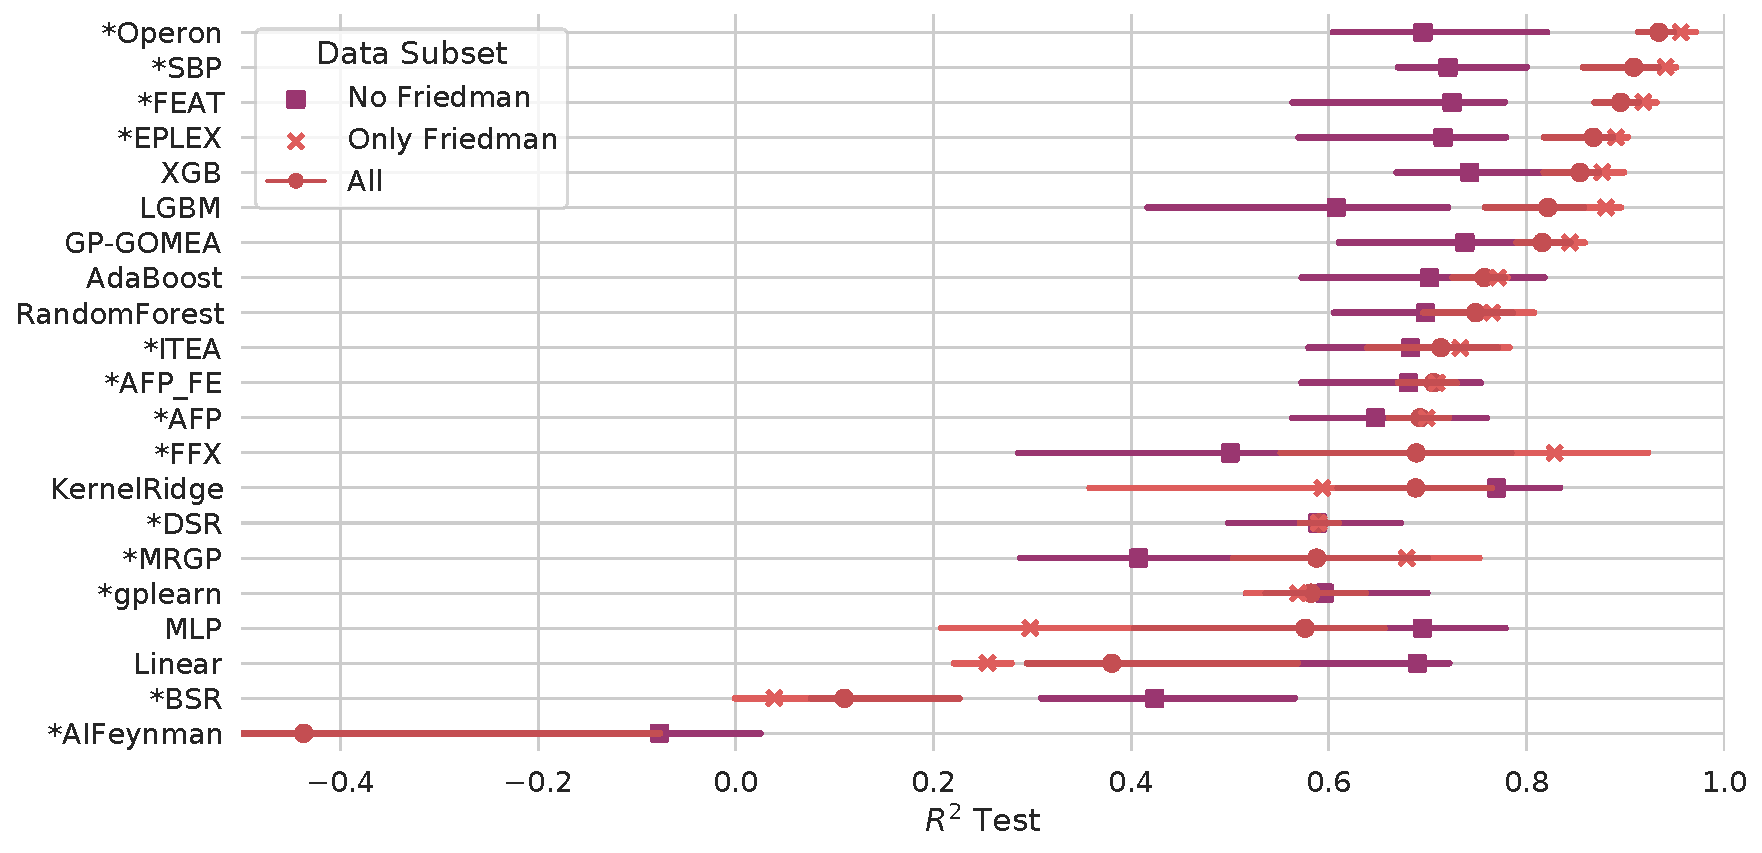
\includegraphics[width=\textwidth]{figs/results_pmlb_r1/friedman_comparison_pairgrid-pointplot_r2_test.pdf}

    \caption{
        Comparison of normalized $R^2$ test scores on all black-box datasets, just the Friedman datatasets, and just the non-Friedman datasets.
    }
    \label{fig:friedman}
\end{figure}


\subsection{Statistical Tests}
Figures~\ref{fig:heat_stats_bb}-\ref{fig:heat_stats_sr} give summary significance levels of pairwise tests of significance between estimators on the black-box and ground-truth problems. 
All pair-wise statistical tests are Wilcoxon signed-rank tests. 
A Bonferroni correction was applied, yielding the $\alpha$ levels given in each. 
This methodology for assessing statistical significance is based on the recommendations of~\citet{demsarStatisticalComparisonsClassifiers2006a} for comparing multiple estimators over many datasets.
These figures are intended to complement Figures~\ref{fig:pmlb_perf}-\ref{fig:symbolic_solns} in which effect sizes are shown. 

\begin{figure}
    \begin{minipage}{0.5\textwidth}
        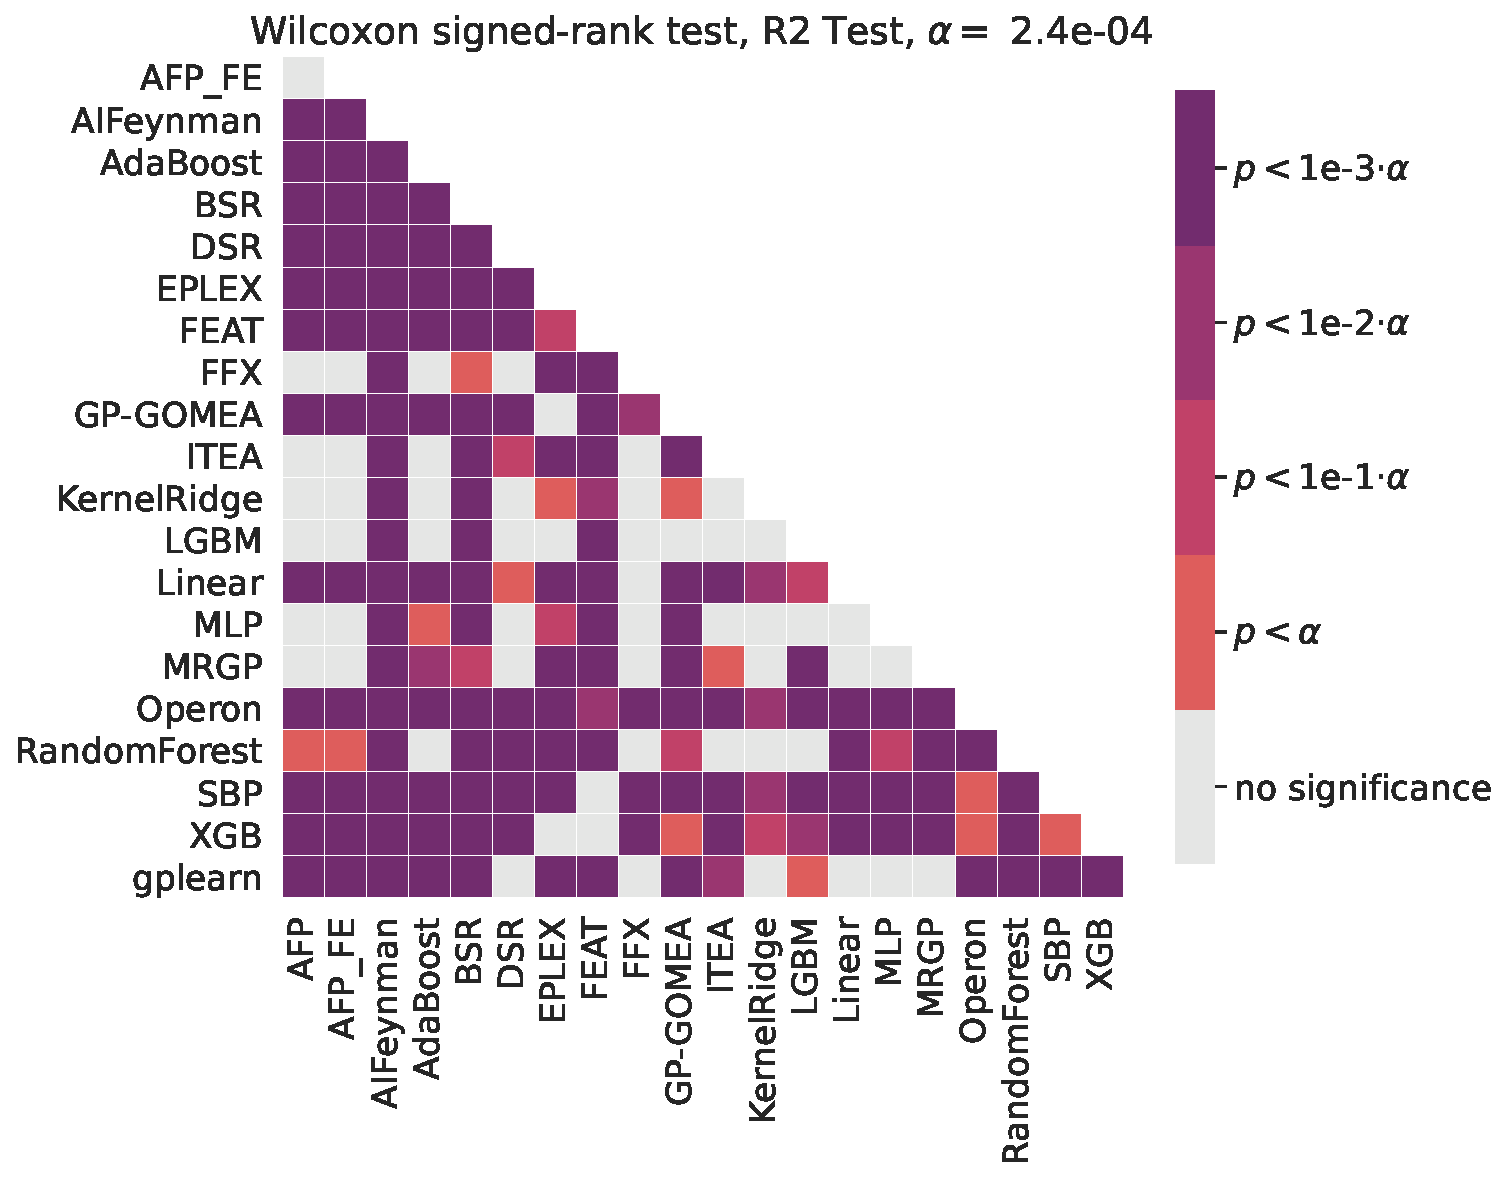
\includegraphics[width=\textwidth]{figs/Pairwise_comparison_of_R2_Test_on_black-box_problems.pdf}
    \end{minipage}
    % \hspace{0.02\textwidth}
    \begin{minipage}{0.5\textwidth}

        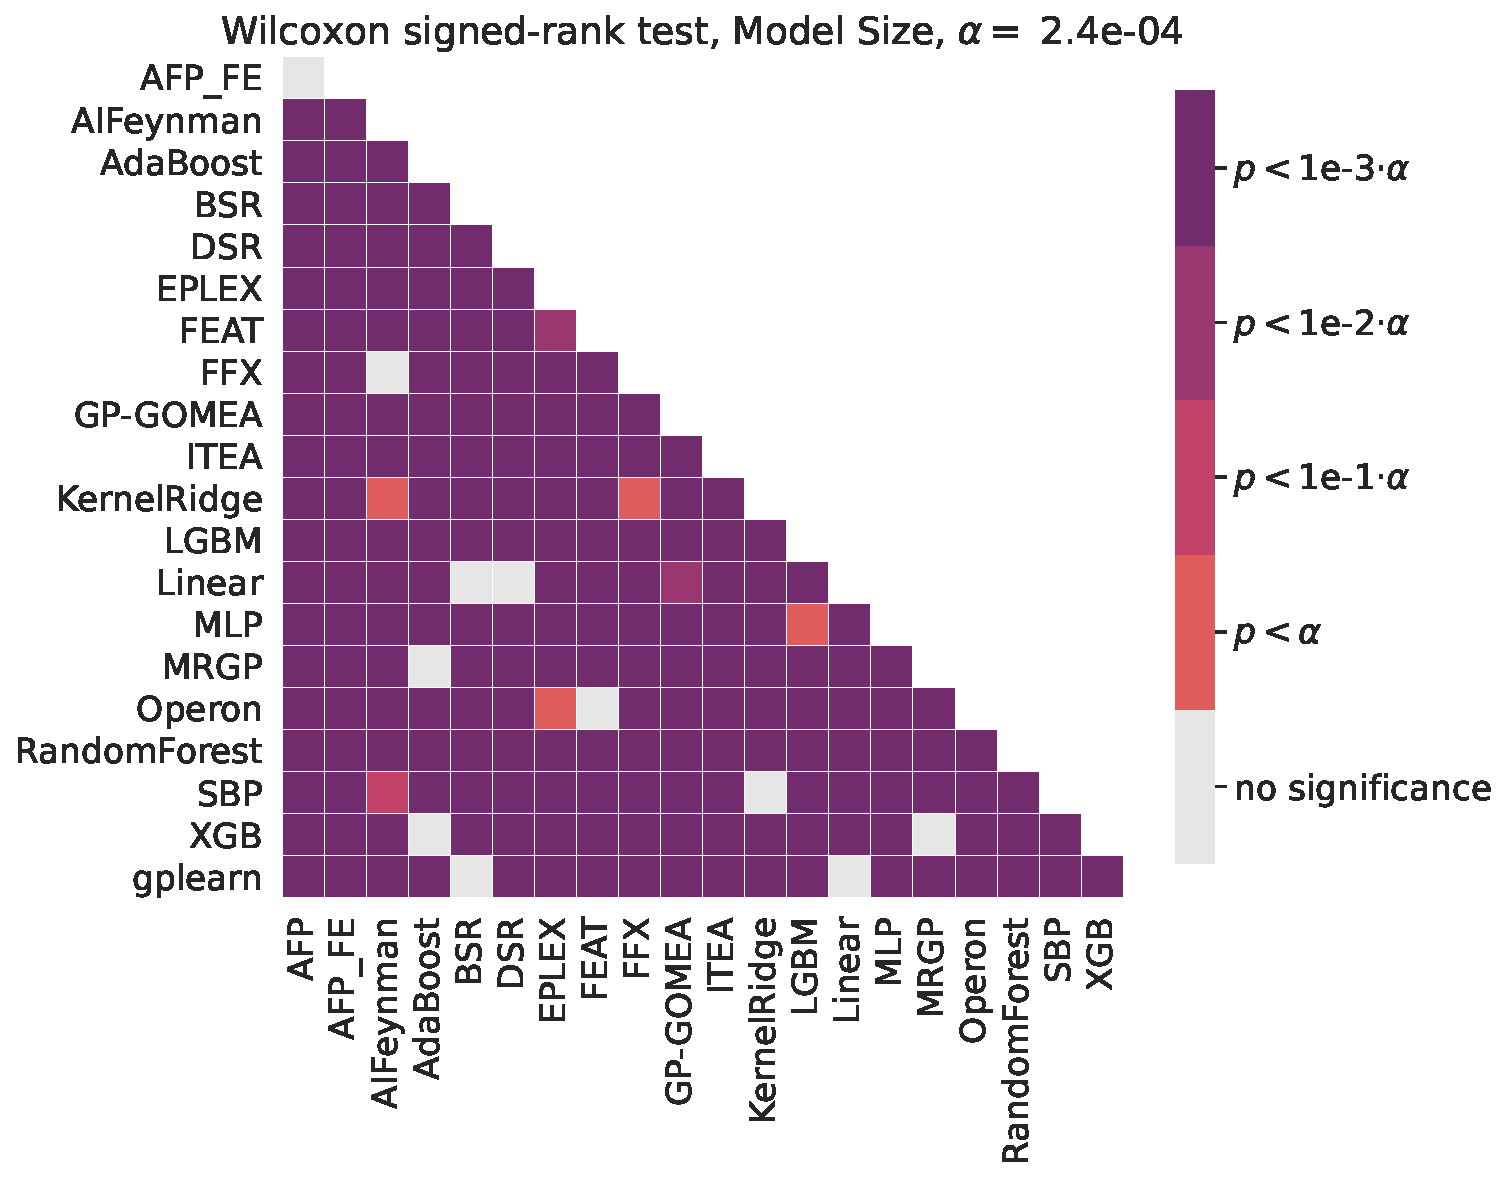
\includegraphics[width=\textwidth]{figs/Pairwise_comparison_of_Model_Size_on_black-box_problems.pdf}
    \end{minipage}
        \caption{ 
            Pairwise statistical comparisons on the black-box regression problems. 
            Wilcoxon signed-rank tests are used with a Bonferonni correction on $\alpha$ for multiple comparisons.
            (Left) $R^2$ test scores, (Right) model size. 
        }
        \label{fig:heat_stats_bb}
\end{figure}




\begin{figure}
    \begin{minipage}{0.5\textwidth}
        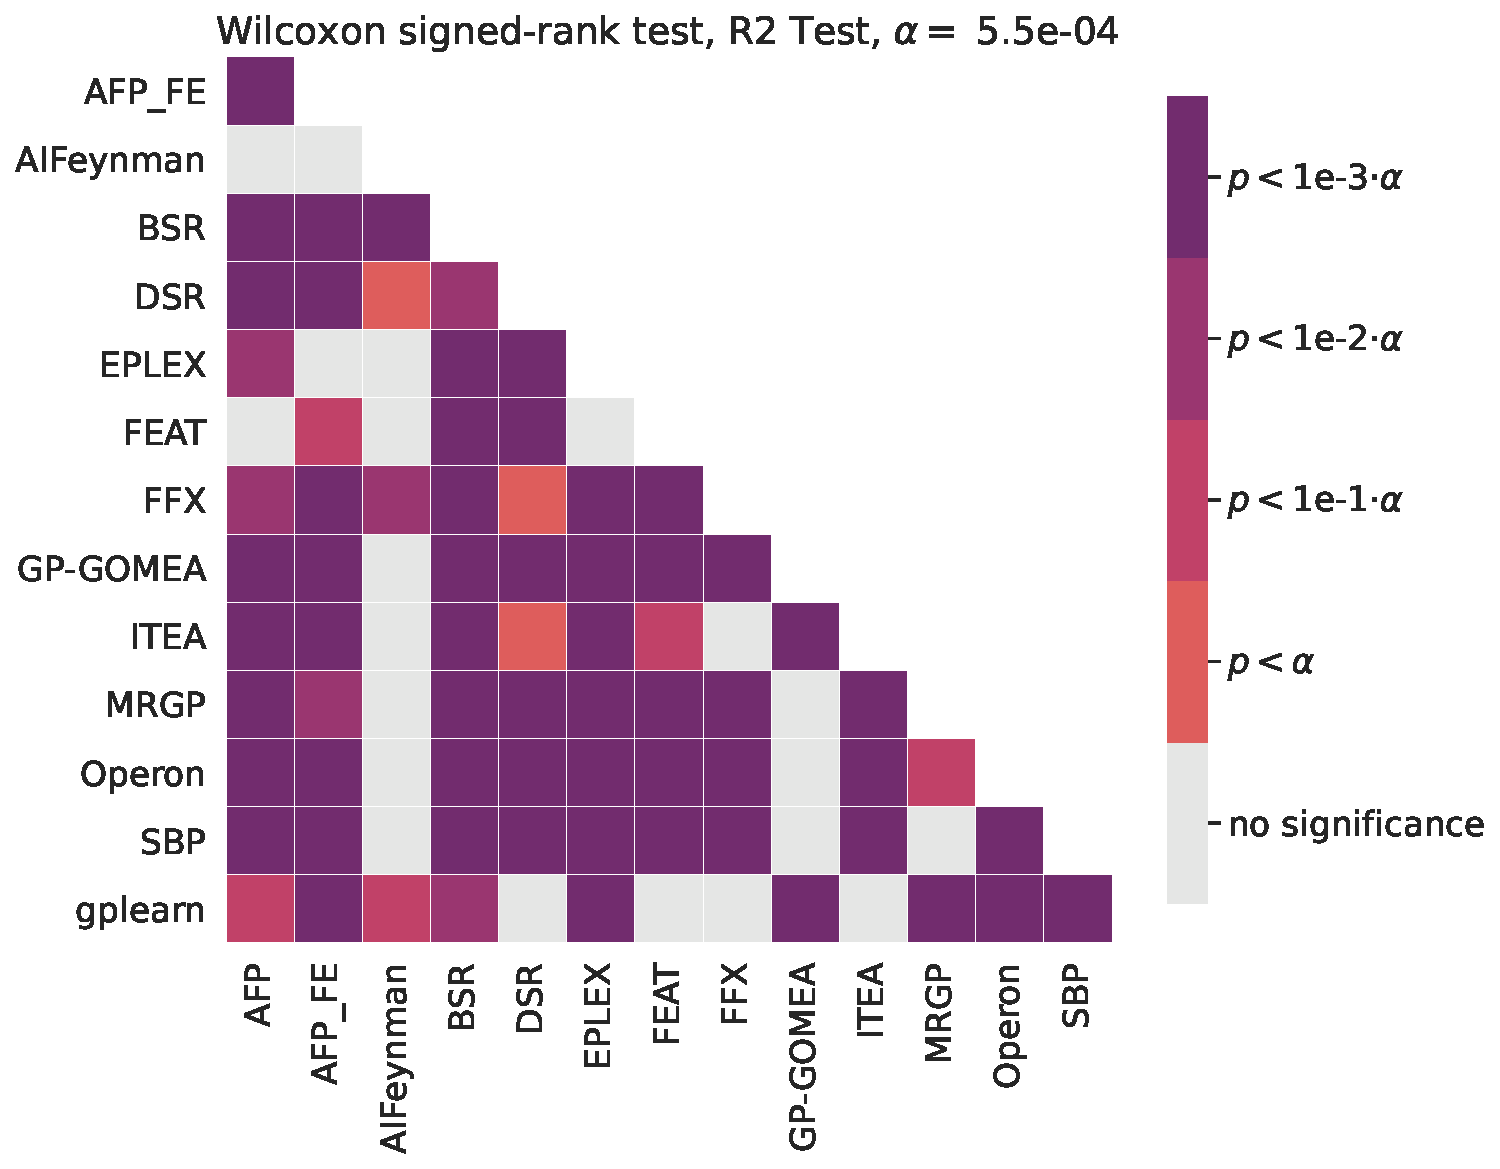
\includegraphics[width=\textwidth]{figs/Pairwise_comparison_of_R2_Test_on_symbolic_problems_target_noise=0.0.pdf}
    \end{minipage}
    % \hspace{0.02\textwidth}
    \begin{minipage}{0.5\textwidth}
        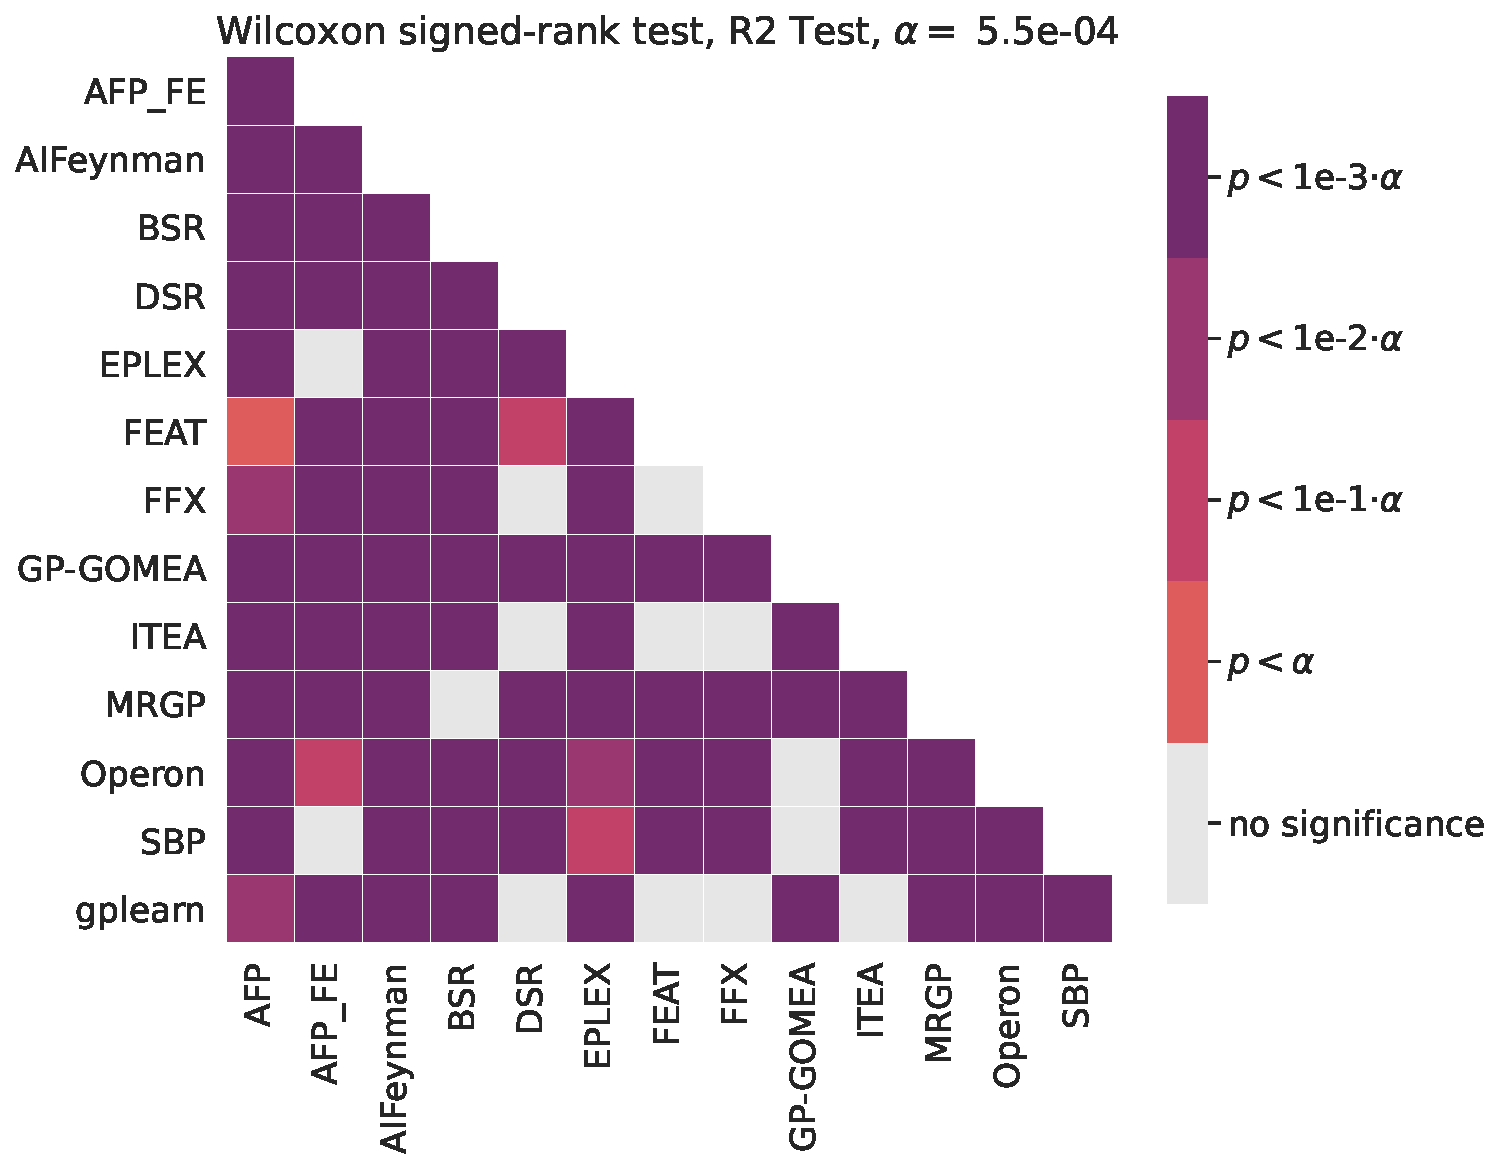
\includegraphics[width=\textwidth]{figs/Pairwise_comparison_of_R2_Test_on_symbolic_problems_target_noise=0.001.pdf}
    \end{minipage}
    \caption{ 
        Pairwise statistical comparisons of $R^2$ test scores on the ground-truth regression problems. 
        We report Wilcoxon signed-rank tests with a Bonferonni correction on $\alpha$ for multiple comparisons.
        (Left) target noise of 0, (Right) target noise of 0.001. 
    }
    \label{fig:heat_stats_r2_sr}
\end{figure}

\begin{figure}
    \begin{minipage}{0.5\textwidth}
        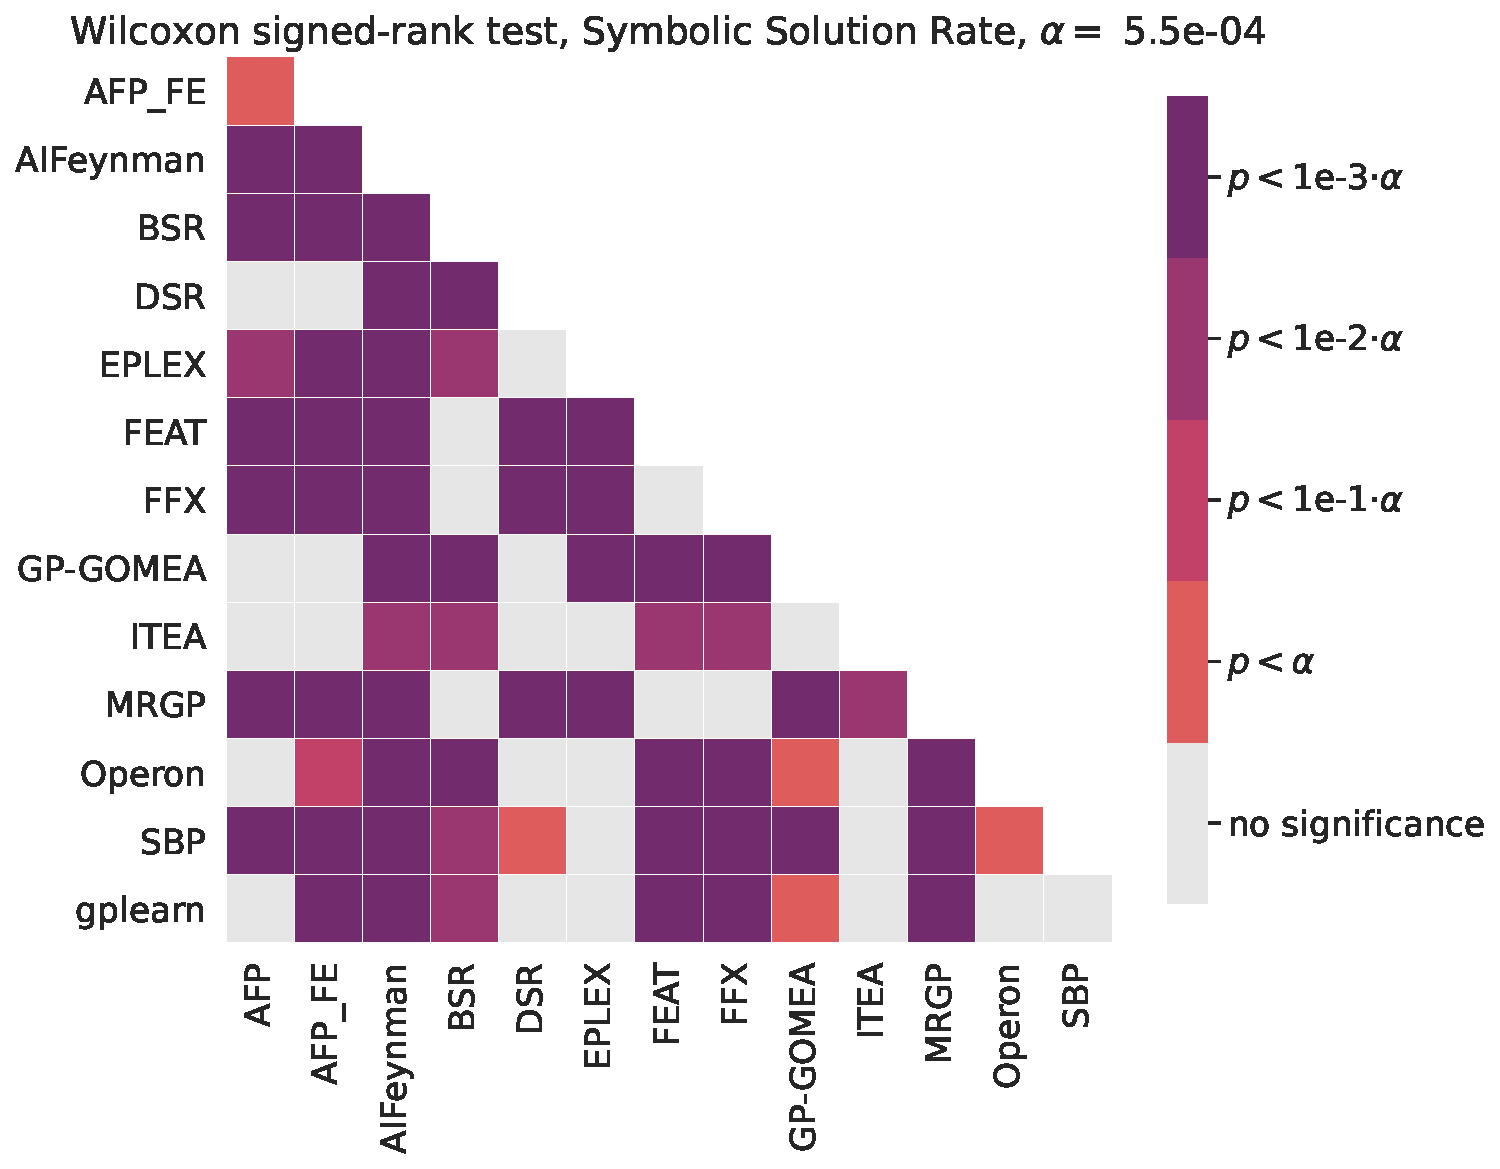
\includegraphics[width=\textwidth]{figs/Pairwise_comparison_of_Symbolic_Solution_Rate_on_symbolic_problems_target_noise=0.0.pdf}
    \end{minipage}
    \begin{minipage}{0.5\textwidth}
        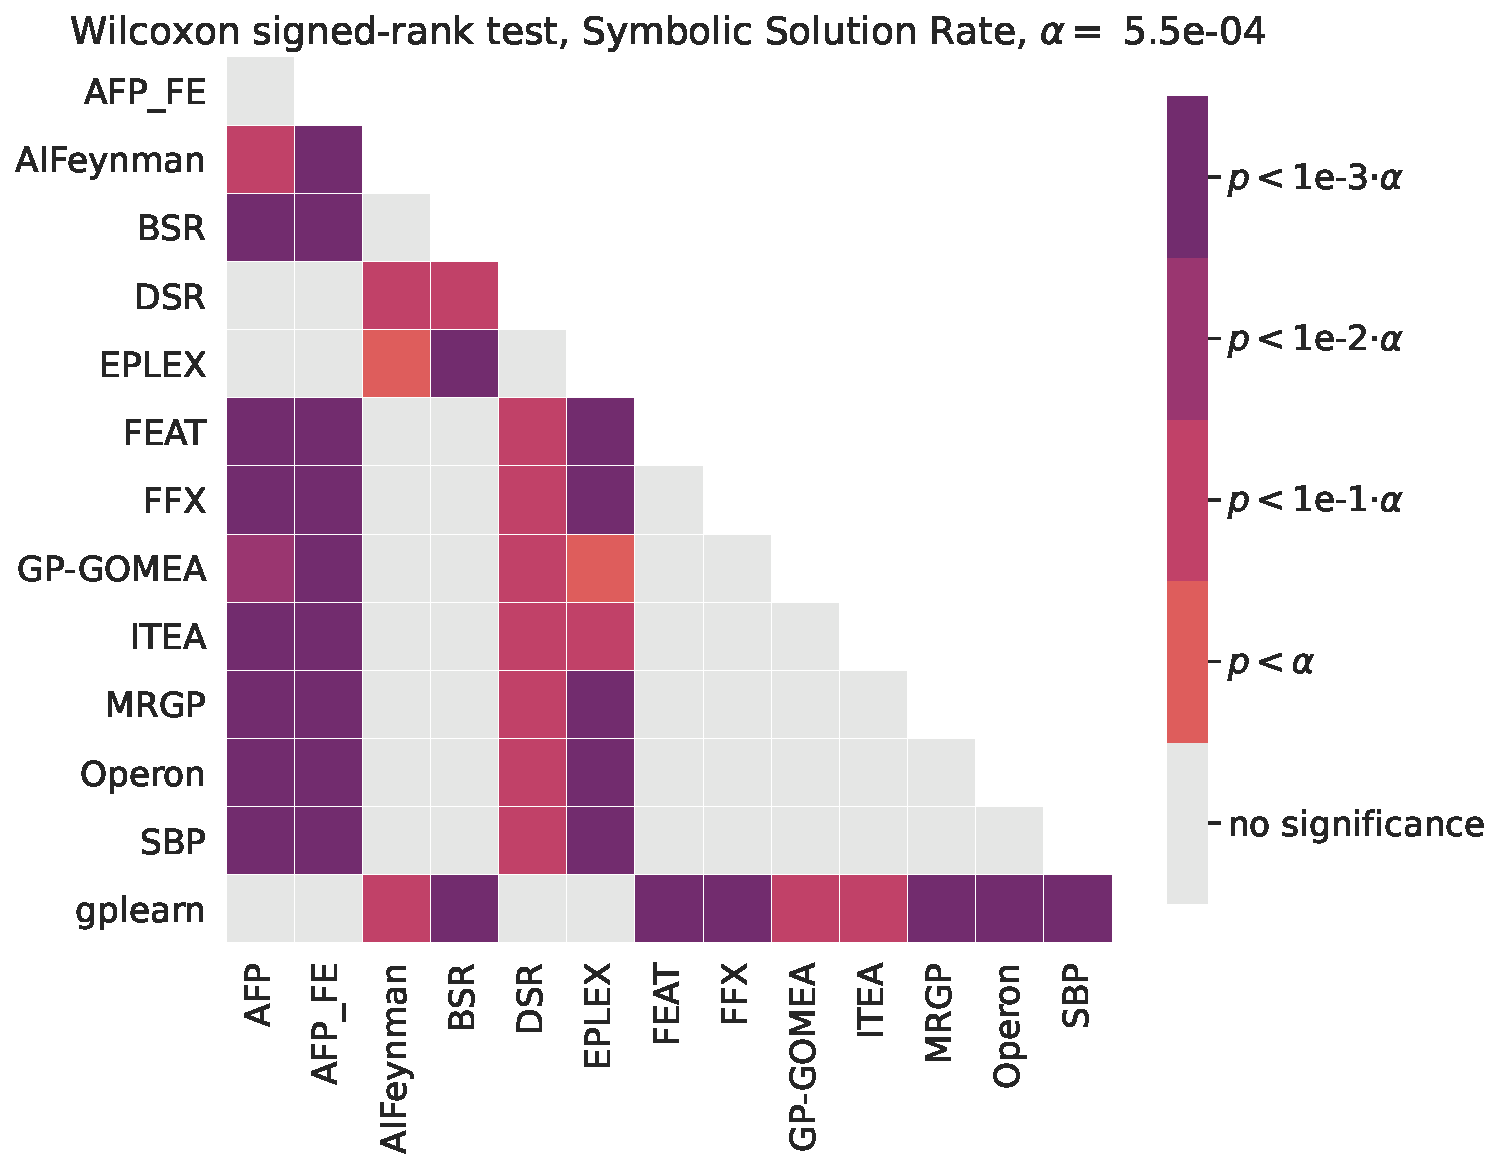
\includegraphics[width=\textwidth]{figs/Pairwise_comparison_of_Symbolic_Solution_Rate_on_symbolic_problems_target_noise=0.001.pdf}
    \end{minipage}
    \caption{ 
        Pairwise statistical comparisons of solution rates on the ground-truth regression problems. 
        We report Wilcoxon signed-rank tests with a Bonferonni correction on $\alpha$ for multiple comparisons.
        (Left) target noise of 0, (Right) target noise of 0.001. 
    }
    \label{fig:heat_stats_r2_sr}
\end{figure}

% \begin{table}
%     \centering
%     \tiny 
%     \input{tables/all_black_box_r2_test.tex}
% \end{table}
% \resizebox{\textwidth}{!}{%
% \begin{table}
\centering
\tiny
\caption{Pairwise comparisons of R2 Test across the symbolic datasets. Bold indicates significant differences ($p<\alpha$, $\alpha=$0.0005).}
\begin{tabular}{llllllllllllll}
\toprule
alg2 &           AFP\_FE &        AIFeynman &              BSR &              DSR &            EPLEX &             FEAT &              FFX &         GP-GOMEA &             ITEA &             MRGP &           Operon &              SBP &          gplearn \\
alg1      &                  &                  &                  &                  &                  &                  &                  &                  &                  &                  &                  &                  &                  \\
\midrule
AFP       &  \textbf{6.9e-31} &  \textbf{8.5e-38} &    \textbf{4e-57} &  \textbf{2.9e-46} &            0.096 &  \textbf{1.7e-21} &  \textbf{1.7e-27} &  \textbf{3.1e-25} &  \textbf{9.1e-28} &  \textbf{7.1e-33} &  \textbf{1.1e-10} &          0.00055 &  \textbf{1.8e-18} \\
AFP\_FE    &                - &  \textbf{3.8e-39} &  \textbf{1.4e-62} &  \textbf{2.9e-49} &  \textbf{3.8e-05} &  \textbf{2.3e-38} &  \textbf{4.7e-46} &  \textbf{4.6e-13} &  \textbf{1.1e-40} &  \textbf{2.6e-40} &             0.12 &            0.023 &  \textbf{9.9e-42} \\
AIFeynman &                - &                - &  \textbf{1.4e-27} &  \textbf{8.4e-36} &  \textbf{5.5e-38} &  \textbf{1.6e-34} &  \textbf{1.2e-34} &  \textbf{9.6e-42} &  \textbf{3.9e-36} &    \textbf{5e-08} &  \textbf{1.2e-38} &  \textbf{1.4e-39} &    \textbf{3e-36} \\
BSR       &                - &                - &                - &  \textbf{7.4e-30} &    \textbf{1e-53} &  \textbf{1.5e-48} &  \textbf{2.6e-53} &  \textbf{7.2e-64} &  \textbf{3.5e-41} &  \textbf{2.4e-06} &  \textbf{4.5e-60} &  \textbf{7.9e-58} &  \textbf{1.5e-24} \\
DSR       &                - &                - &                - &                - &  \textbf{8.8e-33} &             0.15 &  \textbf{2.7e-05} &  \textbf{9.3e-46} &  \textbf{1.1e-10} &  \textbf{4.2e-19} &    \textbf{2e-35} &  \textbf{3.4e-29} &  \textbf{3.5e-06} \\
EPLEX     &                - &                - &                - &                - &                - &  \textbf{3.6e-31} &  \textbf{7.9e-27} &  \textbf{2.7e-24} &  \textbf{1.9e-18} &    \textbf{6e-36} &  \textbf{8.8e-13} &  \textbf{0.00013} &  \textbf{1.7e-17} \\
FEAT      &                - &                - &                - &                - &                - &                - &            0.078 &  \textbf{2.2e-50} &            0.038 &  \textbf{1.8e-28} &  \textbf{7.3e-48} &  \textbf{1.4e-36} &            0.098 \\
FFX       &                - &                - &                - &                - &                - &                - &                - &  \textbf{9.4e-60} &             0.13 &  \textbf{2.4e-23} &  \textbf{2.3e-40} &  \textbf{5.1e-26} &             0.41 \\
GP-GOMEA  &                - &                - &                - &                - &                - &                - &                - &                - &  \textbf{3.8e-40} &  \textbf{3.8e-50} &    \textbf{6e-13} &  \textbf{3.4e-25} &  \textbf{1.3e-44} \\
ITEA      &                - &                - &                - &                - &                - &                - &                - &                - &                - &  \textbf{1.5e-21} &  \textbf{2.9e-26} &  \textbf{9.6e-18} &             0.93 \\
MRGP      &                - &                - &                - &                - &                - &                - &                - &                - &                - &                - &  \textbf{4.3e-55} &  \textbf{1.1e-47} &  \textbf{6.6e-22} \\
Operon    &                - &                - &                - &                - &                - &                - &                - &                - &                - &                - &                - &  \textbf{2.6e-45} &  \textbf{4.4e-28} \\
SBP       &                - &                - &                - &                - &                - &                - &                - &                - &                - &                - &                - &                - &  \textbf{9.3e-17} \\
\bottomrule
\end{tabular}
\end{table}

% \begin{table}
\centering
\tiny
\caption{Pairwise comparisons of Simplified Complexity across the symbolic datasets. Bold indicates significant differences ($p<\alpha$, $\alpha=$0.0005).}
\begin{tabular}{llllllllllllll}
\toprule
alg2 &           AFP\_FE &        AIFeynman &              BSR &              DSR &            EPLEX &             FEAT &              FFX &         GP-GOMEA &             ITEA &             MRGP &           Operon &              SBP &          gplearn \\
alg1      &                  &                  &                  &                  &                  &                  &                  &                  &                  &                  &                  &                  &                  \\
\midrule
AFP       &  \textbf{5.5e-10} &  \textbf{3.8e-10} &          0.00075 &  \textbf{2.4e-47} &  \textbf{1.9e-07} &  \textbf{5.2e-11} &    \textbf{7e-61} &  \textbf{2.2e-13} &  \textbf{3.6e-53} &  \textbf{5.3e-65} &  \textbf{1.1e-46} &  \textbf{3.3e-62} &  \textbf{7.4e-06} \\
AFP\_FE    &                - &  \textbf{1.3e-10} &             0.14 &  \textbf{2.4e-50} &             0.57 &  \textbf{3.9e-05} &  \textbf{1.3e-57} &           0.0069 &  \textbf{2.7e-52} &  \textbf{7.2e-65} &  \textbf{1.2e-42} &  \textbf{5.3e-62} &  \textbf{4.4e-09} \\
AIFeynman &                - &                - &  \textbf{1.5e-13} &            0.032 &  \textbf{1.3e-11} &  \textbf{7.3e-14} &  \textbf{1.3e-39} &  \textbf{1.8e-12} &             0.03 &  \textbf{2.5e-60} &  \textbf{1.4e-18} &  \textbf{1.8e-37} &            0.003 \\
BSR       &                - &                - &                - &  \textbf{3.2e-61} &           0.0047 &  \textbf{1.1e-07} &  \textbf{1.6e-59} &  \textbf{1.2e-05} &  \textbf{8.2e-62} &  \textbf{5.1e-65} &  \textbf{1.8e-42} &  \textbf{1.1e-60} &  \textbf{1.6e-09} \\
DSR       &                - &                - &                - &                - &  \textbf{1.8e-51} &  \textbf{2.8e-46} &  \textbf{3.5e-64} &  \textbf{6.7e-55} &  \textbf{0.00014} &  \textbf{2.4e-65} &  \textbf{1.9e-60} &    \textbf{4e-63} &  \textbf{7.8e-12} \\
EPLEX     &                - &                - &                - &                - &                - &  \textbf{1.9e-08} &  \textbf{4.3e-60} &             0.19 &  \textbf{4.2e-50} &  \textbf{2.7e-63} &  \textbf{1.1e-25} &  \textbf{1.4e-59} &  \textbf{1.6e-11} \\
FEAT      &                - &                - &                - &                - &                - &                - &  \textbf{1.2e-56} &           0.0093 &  \textbf{5.4e-47} &  \textbf{3.2e-58} &  \textbf{4.7e-06} &  \textbf{4.7e-52} &  \textbf{6.6e-16} \\
FFX       &                - &                - &                - &                - &                - &                - &                - &  \textbf{2.1e-54} &  \textbf{4.8e-65} &    \textbf{1e-51} &  \textbf{3.3e-44} &            0.002 &  \textbf{5.2e-53} \\
GP-GOMEA  &                - &                - &                - &                - &                - &                - &                - &                - &  \textbf{4.9e-55} &  \textbf{3.5e-65} &  \textbf{1.7e-45} &    \textbf{5e-62} &    \textbf{3e-11} \\
ITEA      &                - &                - &                - &                - &                - &                - &                - &                - &                - &  \textbf{2.3e-65} &  \textbf{5.2e-60} &    \textbf{3e-63} &  \textbf{1.9e-07} \\
MRGP      &                - &                - &                - &                - &                - &                - &                - &                - &                - &                - &  \textbf{2.3e-64} &  \textbf{1.7e-52} &  \textbf{2.5e-62} \\
Operon    &                - &                - &                - &                - &                - &                - &                - &                - &                - &                - &                - &  \textbf{9.5e-59} &  \textbf{5.7e-26} \\
SBP       &                - &                - &                - &                - &                - &                - &                - &                - &                - &                - &                - &                - &  \textbf{9.7e-53} \\
\bottomrule
\end{tabular}
\end{table}

% \input{tables/pvals_bb_r2_test.tex}
% \input{tables/pvals_bb_model_size.tex}

% \begin{table}
\centering
\caption{Pairwise comparisons of Solution Rate (%) across the symbolic datasets. Bold indicates $\alpha<$0.00055.}
\begin{tabular}{llllllllllllll}
\toprule
alg2 & AIFeynman &       BSR &       DSR &     EPLEX &      FEAT &    FE\_AFP &       FFX &   GPGOMEA &      ITEA &      MRGP &    Operon &       SBP &   gplearn \\
alg1      &           &           &           &           &           &           &           &           &           &           &           &           &           \\
\midrule
AFP       &  1.2e-65* &  1.2e-65* &  1.2e-65* &  1.2e-65* &  1.2e-65* &  1.2e-65* &  1.2e-65* &  1.2e-65* &  1.2e-65* &  1.2e-65* &  1.2e-65* &  1.2e-65* &  1.2e-65* \\
AIFeynman &         - &  1.2e-65* &  1.2e-65* &  1.2e-65* &  1.2e-65* &  1.2e-65* &  1.2e-65* &  1.2e-65* &  1.2e-65* &  1.2e-65* &  1.2e-65* &  1.2e-65* &  1.2e-65* \\
BSR       &         - &         - &  1.2e-65* &  1.2e-65* &  1.2e-65* &  1.2e-65* &  1.2e-65* &  1.2e-65* &  1.2e-65* &  1.2e-65* &  1.2e-65* &  1.2e-65* &  1.2e-65* \\
DSR       &         - &         - &         - &  1.2e-65* &  1.2e-65* &  1.2e-65* &  1.2e-65* &  1.2e-65* &  1.2e-65* &  1.2e-65* &  1.2e-65* &  1.2e-65* &  1.2e-65* \\
EPLEX     &         - &         - &         - &         - &  1.2e-65* &  1.2e-65* &  1.2e-65* &  1.2e-65* &  1.2e-65* &  1.2e-65* &  1.2e-65* &  1.2e-65* &  1.2e-65* \\
FEAT      &         - &         - &         - &         - &         - &  1.2e-65* &  1.2e-65* &  1.2e-65* &  1.2e-65* &  1.2e-65* &  1.2e-65* &  1.2e-65* &  1.2e-65* \\
FE\_AFP    &         - &         - &         - &         - &         - &         - &  1.2e-65* &  1.2e-65* &  1.2e-65* &  1.2e-65* &  1.2e-65* &  1.2e-65* &  1.2e-65* \\
FFX       &         - &         - &         - &         - &         - &         - &         - &  1.2e-65* &  1.2e-65* &  1.2e-65* &  1.2e-65* &  1.2e-65* &  1.2e-65* \\
GPGOMEA   &         - &         - &         - &         - &         - &         - &         - &         - &  1.2e-65* &  1.2e-65* &  1.2e-65* &  1.2e-65* &  1.2e-65* \\
ITEA      &         - &         - &         - &         - &         - &         - &         - &         - &         - &  1.2e-65* &  1.2e-65* &  1.2e-65* &  1.2e-65* \\
MRGP      &         - &         - &         - &         - &         - &         - &         - &         - &         - &         - &  1.2e-65* &  1.2e-65* &  1.2e-65* \\
Operon    &         - &         - &         - &         - &         - &         - &         - &         - &         - &         - &         - &  1.2e-65* &  1.2e-65* \\
SBP       &         - &         - &         - &         - &         - &         - &         - &         - &         - &         - &         - &         - &  1.2e-65* \\
\bottomrule
\end{tabular}
\end{table}

% }
% \end{table}


%SOME deleted stuff

%are represented as a list of terms and each term is a tuple containing the transformation function and a list of exponents for the polynomial equation ~\cite{defrancaGreedySearchTree2018,defrancaInteractionTransformationEvolutionaryAlgorithm2020}.
%following Eq.~\ref{eq:interaction}.
%The mutation operators can either add or remove a term, replace the exponent of a variable on a random term, create a new term through positive or negative interaction. 
%The positive interaction is the product of two interaction functions, while negative interaction is the division between two interactions. 
%performs an Ordinary Least Square to adjust the coefficients to the training set.



%Semantic backpropagation (\textbf{SBP}) is a technique invented and popularized by~\cite{wieloch2013running,krawiec2013approximating,pawlak2014semantic} to compute, for a given target value and a tree node position, what output is needed at the given position to make the output of the tree match the target value. It works by iterative inversions of the ancestry of function nodes, from the root down to the chosen node position. 
%Here, we consider the GP algorithm by~\citet{virgolinLinearScalingSemantic2019}, which is an extension of~\cite{wieloch2013running}. 
%To variate programs, SBP is performed on a random node position using the label as target, and the subtree rooted at the sampled node position is replaced with a tree chosen from a pre-computed library. 
%The chosen tree has output that best matches the one computed by SBP (i.e., using the Euclidean distance on output vectors defined over the training set), after applying the optimal affine transformation on its output.




%Symbolic model encoding

%Interaction-Transformation (IT)~\cite{defrancaGreedySearchTree2018,defrancaInteractionTransformationEvolutionaryAlgorithm2020} is another equation representation that constraints the search space to the functional forms following:
%\begin{equation}
%f(\mathbf{x}) = w_0 + \sum_{i}{w_i \cdot (t_i \circ p_i) (\mathbf{x})},
%\label{eq:appfunction}
%\end{equation}
%\noindent where $w_i \in \mathbb{R}$ are adjustable coefficients, $t_i : \mathbb{R} \rightarrow \mathbb{R}$ is the transformation function
%(e.g., $\sin, \tanh, \mathrm{sqrt}$), and $p_i: \mathbb{R}^{d} \rightarrow \mathbb{R}$ for $d$ input variables is the interaction function:
%\begin{equation}
%p(\mathbf{x}) = \prod_{j=1}^{d}{x_j^{k_j}},
%\label{eq:interaction}
%\end{equation}
%\noindent with $k_j \in \mathbb{Z}$ called the \emph{strength} of the interaction


%gene pool optimal mixin
%The goal is to prevent the disruption potentially-salient patterns of components, i.e., \emph{building blocks} with a positive concerted action.
%In~\cite{virgolin2017scalable,virgolin2020improving}, it was shown that GP-GOMEA’s linkage-based recombination works significantly better than random recombination, and is especially competitive when small, potentially interpretable solutions are sought. 
%We use the same implementation of~\cite{virgolin2020improving}.
